%priprava posamezne ure
%tukaj zaporedoma napisemo{st. zaporedne ure}{datum}{naslov}{poglavje}{oblika dela}{pripomocki}
\begin{priprava}{}{}{Integral}{Določeni integral}{frontalna}{tabla}

\didopomba{Začnemo z nečim, kar na prvi pogled nima veze z integralom.}

\naslov{Geometrijski pomen}

Koliko je ploščina območja, ki ga funkcija $ f(x) = x - 1 $ na intervalu $ [2, 4] $ oklepa z $ x $-osjo? \didopomba{Izračunamo iz slikce preko trikotnika in pravokotnika (4).}

\begin{figure}[h]
    \centering
    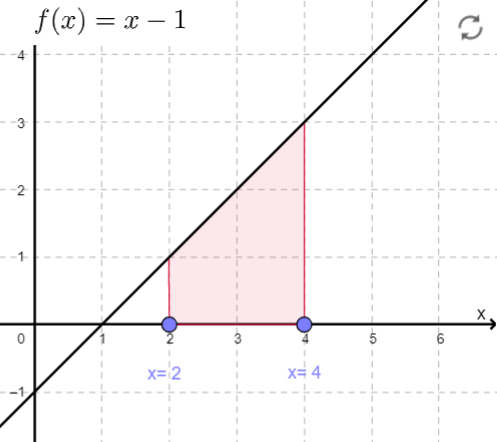
\includegraphics[width=0.4\textwidth]{slike/dol_int_motivacijski_primer.png}
\end{figure}

\didopomba{Zdaj pa si pogledamo aplet na Geogebri (https://www.geogebra.org/m/Fv6t696j), v zvezek si bomo risali potem. Vzamemo drugačno funkcijo: $ f(x) = \sin{2x}+\frac{x^2}{10} + 1 $ na intervalu $ [1,5] $. Kako bi izračunali ploščino pod grafom?}

\begin{figure}[h]
    \centering
    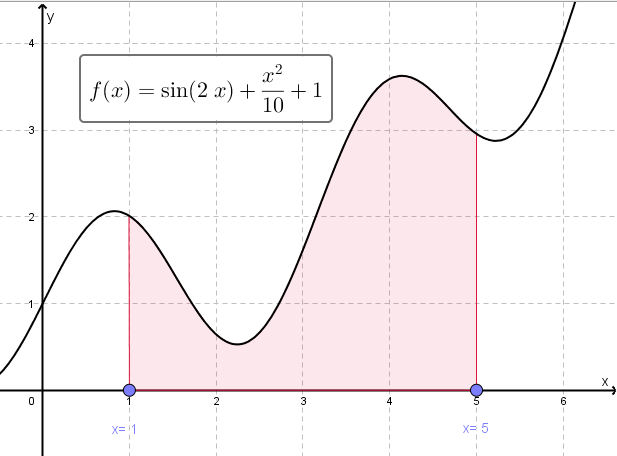
\includegraphics[width=0.3\textwidth]{slike/dol_int_motivacijski_primer2.png}
    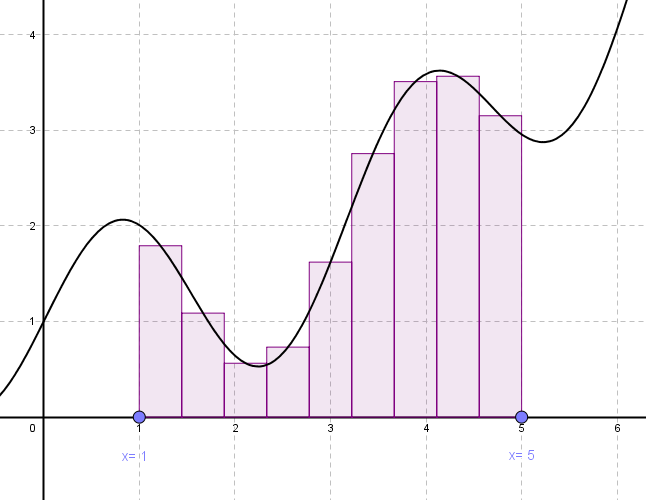
\includegraphics[width=0.3\textwidth]{slike/midpoint.png}
    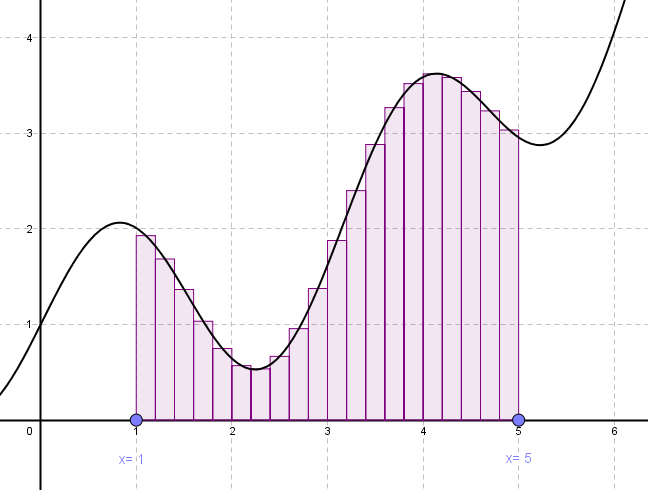
\includegraphics[width=0.3\textwidth]{slike/midpoint2.png}    
\end{figure}


\didopomba{Naj sami predlagajo, da območje razdelimo na znane like, pravokotnike, recimo z enako širino -- ampak s kakšno višino? \\
Torej: Interval razdelimo na enako široke podintervale. Na vsakem pointervalu si izberemo točko, katere vrednost $ f $ bo višina pravokotnika na tem podintervalu. Lahko si izberejo levo/desno mejo podintervalov, ali točko, kjer $ f $ na podintervalu doseže maksimum/minimum, recimo da vzamemo kar točke na sredini podintervalov. \\
Če vzamemo vedno ožje pravokotnike, se vsota ploščin pravokotnikov približuje iskani ploščini.}

\didopomba{Zdaj pa rišemo v zvezek, kot kaže tretja slika (splošna $ f $ na $ [a, b] $). Ploščino lahko zapišemo kot vsoto pravokotnikov s širino $ \Delta x $ in višino $ f(x_i) $, kjer so $ x_i $ sredinske točke $ i $-tega podintervala $ [a, b] $. Več je podintervalov, bolj bo ploščina pravokotnikov podobna pravi ploščini.}

\newpage

\didopomba{Limito vsote označimo z znakom $ \int $ (oznako je uvedel Leibniz); integral je v bistvu ena vsota, kjer se pomikamo po res neskončno majhnih korakih. Pri tem se $ \Delta x $ zamenja z $ dx $, s čimer poudarimo, da gredo širine podintervalov proti 0.}

$$
S = \lim_{n \rightarrow \infty} \sum_{i=1}^n f(x_i) \cdot \Delta x = \int_a^b f(x) dx
$$

$ a $ imenujemo \emph{spodnja meja} integrala, $ b $ pa \emph{zgornja meja}.

\didopomba{Od tu pride oznaka $ \int dx $ pri nedoločenih integralih, ne pa obratno ...}

\textcolor{rdeca}{Določeni integral $ \int_a^b f(x) dx $ je enak ploščini lika, ki je omejen z grafom funkcije $ f $, $ x $-osjo ter premicama $ x = a $ in $ x = b $.}

\begin{figure}[h]
    \centering
    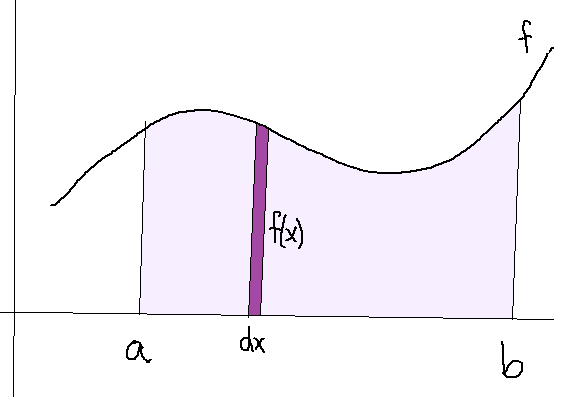
\includegraphics[width=0.4\textwidth]{slike/dol_int_skica.png}
\end{figure}

Pogoj: $ f (x) $ je zvezna in na $ [a, b] $ nenegativna \didopomba{Za zvezno lahko pokažeš, da odsekoma zvezne funkcije ne moreš sploh vpisat v integral. Za negativno pa upoštevaš, da je $ f(x_i) < 0 $, torej je vsota in s tem integral negativen. Ploščina pa je po velikosti enaka (spodnja slika)}.

\didopomba{Poudari, da je dol. integral število (ne pa funkcija)! Zaenkrat ga še ne znamo izračunati, še pride}

\begin{figure}[h]
    \centering
    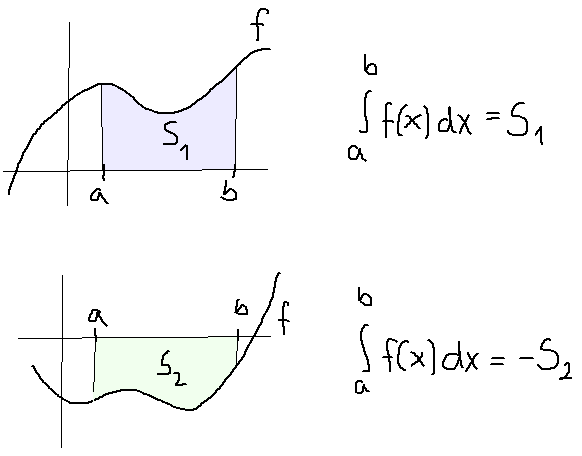
\includegraphics[width=0.5\textwidth]{slike/ploscine.png}
\end{figure}

Kaj pa, če je na $ [a, b] $ funkcija malo pozitivna, malo negativna?

\newpage

\begin{figure}[h]
    \centering
    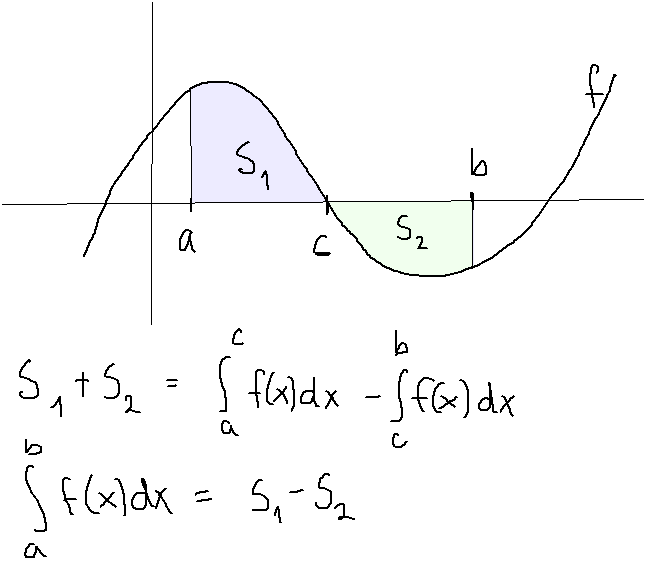
\includegraphics[width=0.5\textwidth]{slike/ploscine2.png}
\end{figure}

Ploščina območja je tako vedno enaka $ S = \int_a^b | f(x) | dx $ ne glede na predznak $ f $.

Kratka vaja \vaje{(npr. slikco s polinomom z znanimi ploščinami, računaš le po eno območje naenkrat, pač enkrat bo +, enkrat -)}:

\begin{figure}[h]
    \centering
    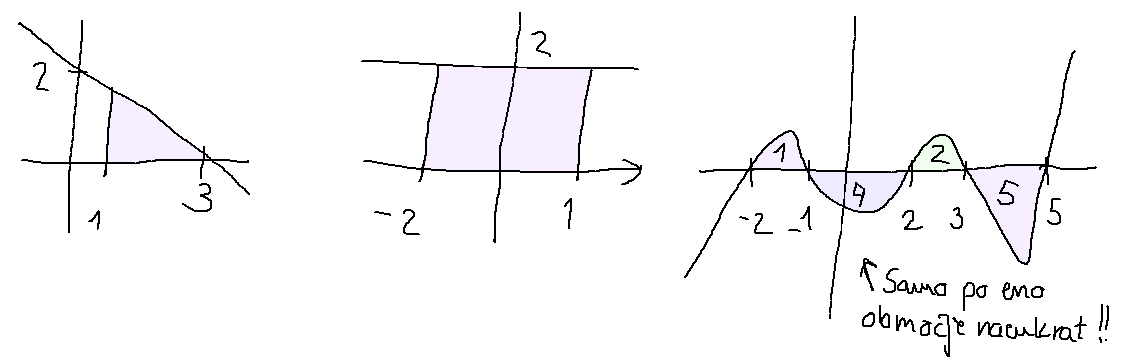
\includegraphics[width=0.9\textwidth]{slike/dol_vaje1.png}
\end{figure}

Potem pa še nekaj logičnih lastnosti \didopomba{sledijo iz ploščine (lahko zraven skice), se jih tudi preveri, ko spoznajo N-L formulo}:

\naslov{Lastnosti}

\didopomba{Lahko si zraven slikco narišeš}

\begin{itemize}
    \item $ \int_a^a f(x) dx = 0 $
    \item $ \int_a^c f(x) dx + \int_c^b f(x) dx = \int_a^b f(x) dx $, kjer je $ c \in [a, b] $
    \item $ \int_a^b f(x) dx = - \int_b^a f(x) dx $ \didopomba{To je bolj dogovor, ampak bo pa očitno sledilo iz NL formule}
    \item $ \int_a^b c \cdot f(x) dx = c \cdot \int_a^b f(x) dx $
    \item $\int_a^b (f(x) + g(x)) dx = \int_a^b f(x) dx + \int_a^b g(x) dx $
    \item Izrek o povprečni vrednosti: $ \int_a^b f(x) dx = (b-a)p \rightarrow $: $ p = \frac{1}{b - a} \int_a^b f(x) dx $

\newpage

\begin{figure}[h]
    \centering
    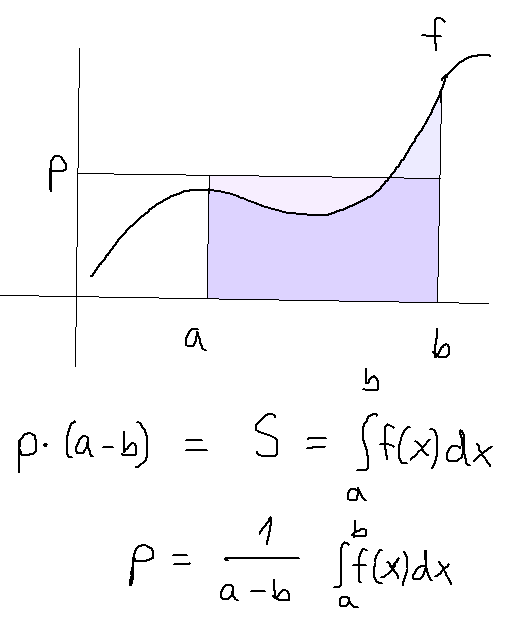
\includegraphics[width=0.4\textwidth]{slike/povprecna_vrednost.png}
\end{figure}

\end{itemize}


\vaje{
Vaje:
\begin{itemize}
    \item Lahko naloge - funckije z znano ploščino (jo znaš razbrati iz grafa, kakšne premice, absolutno, krožnice ...), najprej na enem območju, pozitivno/negativno, nato malo pozitivno in malo negativno
    \item funkcije, kjer se ploščine odštejejo v 0 (npr. lihe funkcije, $ \int_0^{2\pi} \sin x dx $)
    \item sode funkcije na simetričnem intervalu $ [-a, a] $ -- lahko integriraš po $ [0, a] $ in podvojiš! (včasih je to enostavneje, saj vstavljaš v eno mejo 0).
    \subitem tudi $ \int_{-\pi/2}^{pi/2} \cos x dx $ je vredu primer, pač se da poenostavit v $ \int_0^{\pi/2} \cos x dx $.
    \item valovita funkcija z odsekoma znanimi ploščinami (ampak neznanim predpisom) in morajo izračunati določeni integral na različnih intervalih, pa $ 2f(x), -f(x), |f(x)| $ ipd.
    \item Oceni ploščino funkcije (npr. na [0, 2], min = 1 in max = 2 -> ploščina je med 2 in 4. Nato jo še izračunamo.) ALI npr. Za integral $ \int_e^{e^2} \ln x dx $ ugotovi, ali je večji od 2, ali je večji od 30. \didopomba{Naj sami razmislijo, kako se tega lotiti.}
\end{itemize}
}
 
Zdaj pa nam že malo nagaja, ker ne znamo izračunati določenega integrala, drugega primera ($ f(x) = \sin{2x}+\frac{x^2}{10} + 1 $) ne znamo izračunati ...

\naslov{Newton-Leibnizova formula}

Da bomo lahko integral lahko tudi izračunali, si za začetek poglejmo funkcijo na sliki (levo).

\begin{figure}[h]
    \centering
    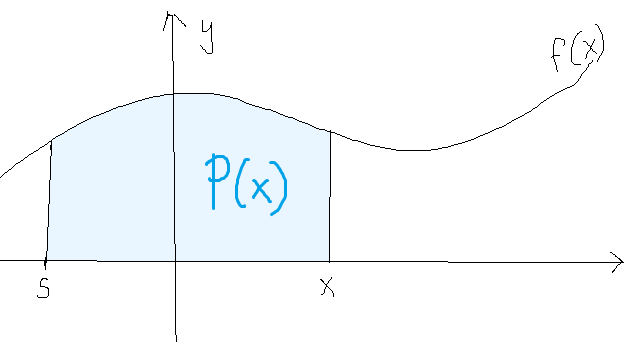
\includegraphics[width=0.45\textwidth]{slike/NL_P(x).png}
    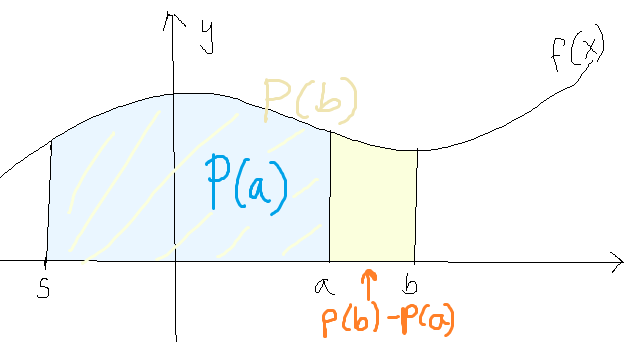
\includegraphics[width=0.45\textwidth]{slike/NL_P(b)-P(a).png}
\end{figure}

\newpage

Funkcija $ P(x) $ pogleda območje med grafom $ f $ in $ x $-osjo na intervalu $ [ s, x] $ \didopomba{$ s $ je pač eno število, NI VAŽNO} in prišteje območje, kjer je $ f $ pozitivna, in odšteje območje, kjer je $ f $ negativna. Tako vidimo, da se $ P $ obnaša ravno tako kot integral:

$$ P(x) = \int_s^x f(t) dt $$

Izrazimo še (očitno sledi iz slike (zgoraj desno)) $ \int_a^b f(x) dx = P(b) - P(a) $. Waw, to pa smo že bližje. Manjka nam samo še predpis za $ P $. Zato si \didopomba{hint} poglejmo njen odvod:

$$
P'(x) = \lim_{h \rightarrow 0} \frac{P(x + h) - P(x)}{h} = \lim_{h \rightarrow 0} \frac{f(x) \cdot h}{h} = f(x)
$$

Pri tem smo iz slike videli, kaj je $ P(x + h) - P(x) $ in ko gre $ h $ proti 0, je višina tega ``pravokotnika'' kar $ f(x) $.

\begin{figure}[h]
    \centering
    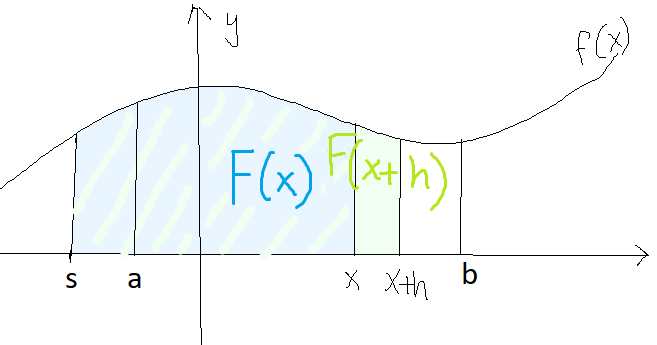
\includegraphics[width=0.5\textwidth]{slike/NL_P(x)_P(x+h).png}
\end{figure}


Že vemo, da $ P'(x) = f(x) $ pomeni, da je $ P(x) $ nedoločen integral funkcije $ f $ ($ \int f(x) dx = P(x) + c $), torej $ P $ dejansko že znamo določiti!

Povzemimo: če \textcolor{rdeca}{$ \int f(x) dx = F(x) + c $}, potem je \textcolor{rdeca}{$\int_a^b f(x) dx = F(x)|_a^b = F(b) - F(a) $} \didopomba{Oznako s $ | $ napiši nazadnje, pač to je krajši zapis. Tu ni več c-jev!} Newton-Leibnizova formula (NL-formula).

Z besedo: Določen integral funkcije je enak razliki vrednosti njenega nedoločenega integrala na zgornji in spodnji meji.

Izračunamo prav ta prvi primer pri določenem integralom še s to formulo: $ \int_2^4 (x - 1) dx = (\frac{x^2}{2} - x) |_2^4 = 4 $.

Pa še drugega: $ \int_1^5 (\sin{2x}+\frac{x^2}{10} + 1) dx = \ldots \approx 8,14 $

\vaje{
Vaje:
\begin{itemize}
    \item Z N-L formulo preveri veljavnost pravil, ki smo jih našteli zgoraj \didopomba{razen povprečne vrednosti}
    \item basic vaje
    \item odsekoma zvezna funkcija \didopomba{Sami pogruntajo, da morajo ločiti na vsoto več integralov}
\end{itemize}
}

\newpage

\naslov{Per partes v nedoločenem integralu}

A je to sploh noter? Sicer pa itak sam dodaš meje.

\naslov{Uvedba nove spremenljivke}

\textcolor{rdeca}{PAZI! Le če je nova spremenljivka monotona funckija, lahko to narediš !! (sicer se ti vmes integral malo odšteje/prišteje \ldots)}

$ \int_1^3 (2x + 1)^5 dx $ lahko rešimo na dva načina:
\begin{itemize}
    \item kot do sedaj (izračun nedoločenega integrala): $ \int (2x + 1)^5 dx = \int \frac{t^5}{2} dt = \frac{(2x + 1)^6}{12} + c $
    \subitem $ \int_1^3 (2x + 1)^5 dx = \frac{(2x + 1)^6}{12} |_1^3 = \ldots = \frac{29230}{3} $
    \item s spremembo meje: $ \int_1^3 (2x + 1)^5 dx = \int_3^7 \frac{t^5}{2} dt = \frac{t^6}{12} |_3^7 = \frac{29230}{3} $
\end{itemize}
\didopomba{Nazorno zapiši pri mejah $ 2 \cdot 1 + 1 = 3 $ itd.}

\vaje{Vaje: Spet nekaj primerov za zamenjavo spremenljivk.}

\end{priprava}